% \part{Introduction}

\section {Introduction}

% task 
% traditional method
% current method
% lack of current method
% main update of your method
% additional output

3D Display System aims to proide immersive and interactive experiences of virtual scenarios base on human vision illusions. Since the concept of metaverse is introduced by Facebook, 3D display technology is attracting more and more attetion from both academic and industrial field.

While earlier 3D display base on binocular vision by allying two images as binocular disparity, the traditional 3D display system usually requires professional photographic capture devices and specialized glasses, which limits the accessibility and convenience of the system. Recent years naked-eye display systems based on horizontal parallax coms into public view. L-shaped monitor on Taiguli Chengdu(Figure 1) is a typical example of horizontal parallax illusion applications, since the shape provide additional depth illusion.\cite{Wang2024} Althought the L-shaped display system excuse users from wearing heavy glasses, the expensive price and fixed position of the viewer still limit its accessibility and convenience.

\begin{figure}[htb]
    \centering
    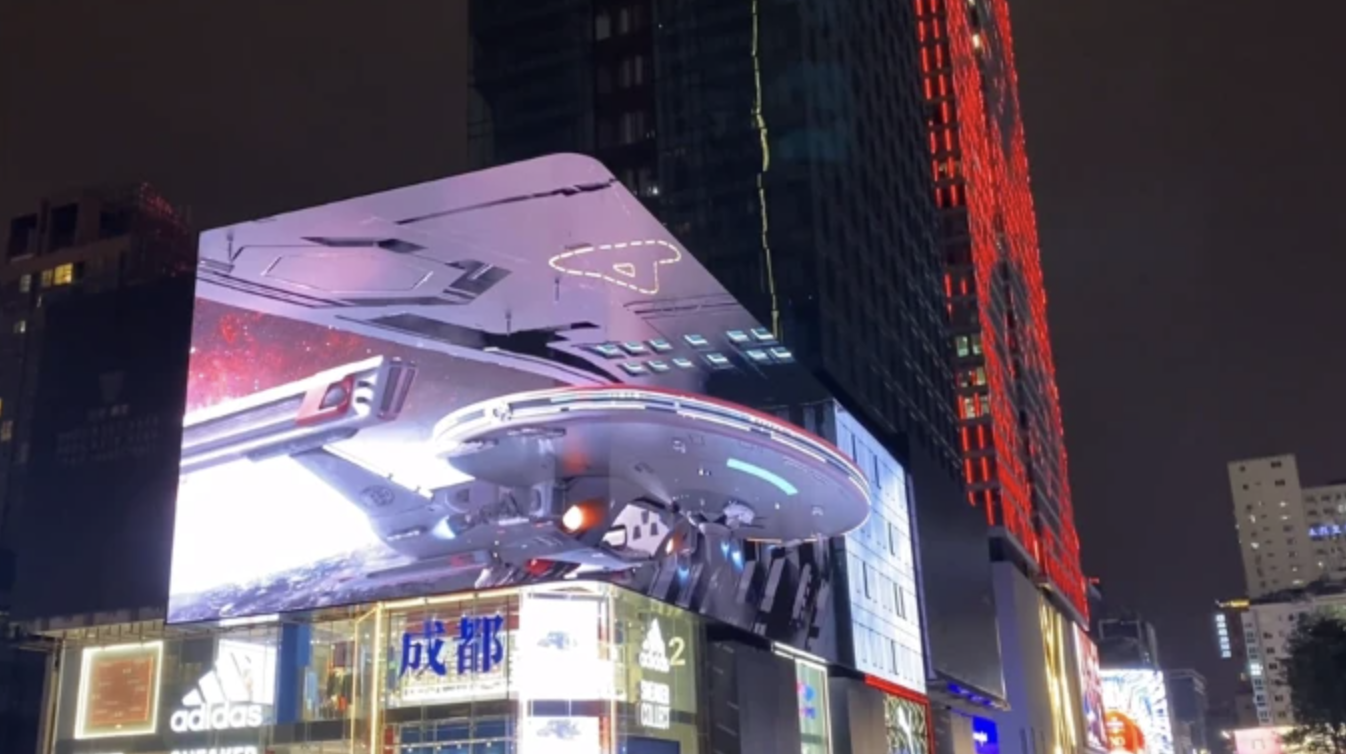
\includegraphics[width=0.7\textwidth]{figures/L-shaped.png}
    \caption{L-shaped display monitor}\label{F:test-a}
\end{figure}

To tackle these problems, another motion parallax based light-weight solution is proposed\cite{ALLISON20031879}. Wang\cite{Wang_2018} introduce a 3D display system based on Kinect SDK, and Peder. 2019 \cite{TheParallaxView} developed an IOS application based on iPhoneX's TrueDepth camera. These two systems both use the combination of head-track and off-axis perspective projection, provided a customer-oriented 3D display system. Compare with L-shaped solutions, motion-based 3D display system is more flexible and cheaper, since it only requires a camera and a display device.

\begin{figure}[htb]
    \centering
    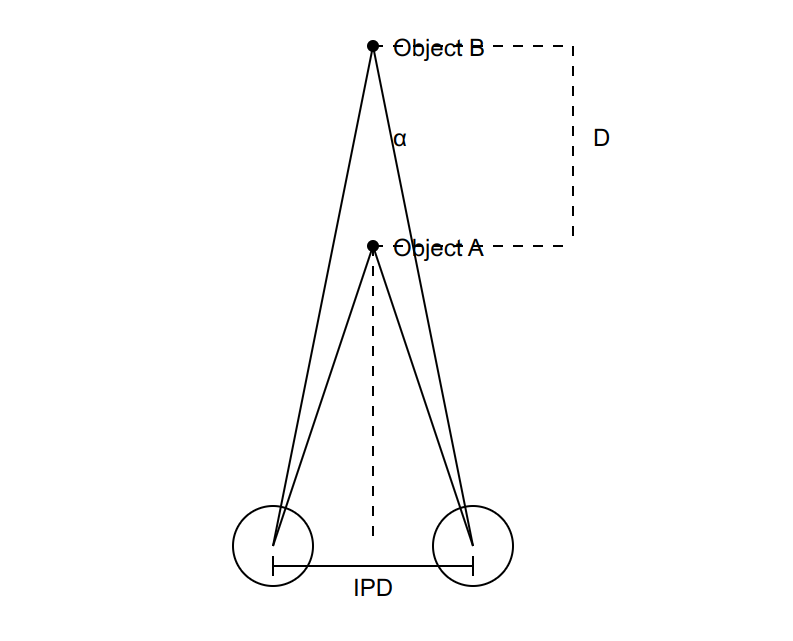
\includegraphics[width=0.6\textwidth]{figures/Introduction/Horizontal.png}
    \caption{Horizontal parallax}\label{F:test-a}
\end{figure}

However, the head-track part in these two systems is essentially using SDK procided by hardware manufacturers(Kinect in Wang's work, and iPhone in Pader's work), which suffers from hardward limitations. Although depth measurement devices exactly provides a more convenience and stable solution, the flexibility and expensibility cannot reach requirements. Consider a general head-track task which need to inference human head's position, given a specific usage scenary, a head-track task requirement usually need to cover difference specific conditions. For example, laptop deployments without an external depth camera or laser radar. Also, SDK-based traking solutions is not flexible enough to handle possible bugs and errors, since the source code is not open to the public, makes it's harder to be mentained by single developer. In additional, SDK-based solution can only be deployed as assemblyies or on specific devices: the former needs extra cost for expensive professional devices, and the latter limits the system's application for different users, which introduce extra cost and limit naked 3d systems' further application.

\begin{figure}[htb]
    \centering
    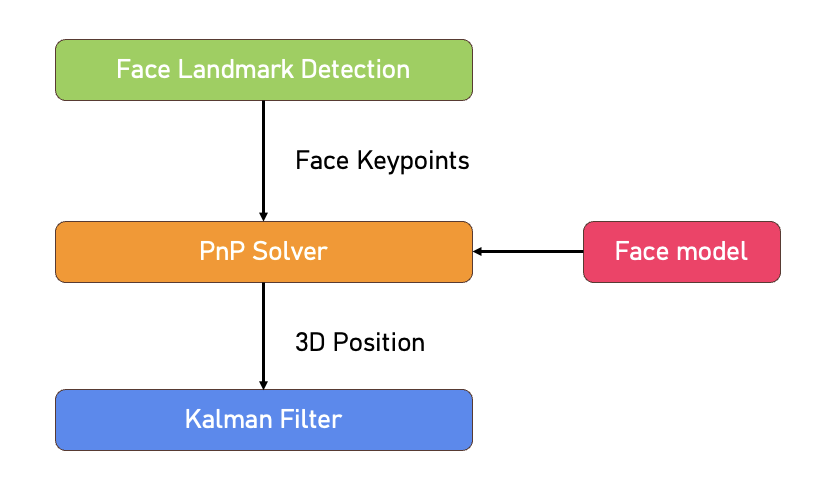
\includegraphics[width=0.8\textwidth]{figures/Introduction/HeadTrack.png}
    \caption{Head tracking system working flow. }\label{F:test-a}
\end{figure}

This work proposed a new head-track solution based on monocular distance measurement and off-axis projection, privide a cheaper and more flexible solution for 3D display system. As shown in figure 3, this work can inference human head's position with a single camera with the support of face landmark detection algotithm and researches of perspective-n-point(PnP) problem, without surpports of depth measurement hardwares. The main update of this work is the combination of face landmark detection and ePnP algorithm\cite{EPnP_2009}, which provide a more flexible and cheaper solution for 3D display system. 

% \begin{figure}[htb]
%     \centering
%     \includegraphics[width=0.5\textwidth]{example-image-a}
%     \caption{Image correction}\label{F:test-a}
% \end{figure}

Beside monocular head-tracking, display optimization is also considered as an important of vision illusions. Since most of motion parallax based 3d systems only consider standard display monitors, we proposed a noval correction algorithm for curved displays. By accepting result from head-traking algorithms, correction algorithm can adjust displayed frames to fit the view angle of users, which is more appropriate for curved displays which is more and more popular in recent years.

The contributions of this work include:

\begin{itemize}
    \item A new head-track system based on monocular distaance measurement, which provide a cheaper and more flexible solution for 3D display system compared with depth-camera based methods.
    \item A correction algorithm for curved displays, which is more appropriate for curved displays which is more and more popular in recent years.
\end{itemize}

In conclusion, this work provides a new head-track system based on monocular distaance measurement, which is more flexible and cheaper than traditional depth-camera based methods. Conbined with off-axis perspective projection and the correction algorithm for curved displays, this work provides a more flexible and cheaper solution for 3D display system.


\clearpage